\section{Analysis}
\label{sec:analysis}

% 注：原 "Analysis and Discussion" 拆分——本节聚焦实证分析（failure taxonomy / grounding depth / distribution），
% "Discussion" 内容移到 §\ref{sec:conclusion} 的 Conclusion 部分。
% 注：原"分析与讨论"已拆分——本节聚焦实证分析（失败分类法 / 接地深度 / 分布），
% "讨论"内容移到第~\ref{sec:conclusion}~节的结论部分。

\subsection{Failure Taxonomy}
\label{sec:failure-taxonomy}
% \subsection{失败分类法}

\textbf{Taxonomy protocol.} We define three mutually exclusive failure modes over the \Neval{} runs: (i) \emph{no-output / aborted}, where the run ends in ERROR (70 runs) or yields no \texttt{submit.zip} (among them the 6 ABSENT runs whose assets were unavailable); (ii) \emph{semantic / partial failure}, where a deliverable exists but at least one reference assertion fails (a subset of the 558 FAIL runs); and (iii) \emph{contract / format failure}, where the content is plausible but file-layout or naming assertions fail. The batch records only the terminal status per run, not which assertion failed first, so the run-level outcome counts we can state with certainty are PASS 62 / FAIL 558 / ERROR 70 / ABSENT 6 of \Neval{}. A systematic per-run labelling pass (\texttt{eval\_triage/05\_batch\_triage.py}, which derives each class from machine-checkable evidence and reports an explicit UNKNOWN share, never folding unclassified runs into another bucket) applied to the per-run judge logs of this batch yields the following measured split over the \Neval{} runs: (i) no-output / aborted = 146/696 = 21.0\% (the 70 ERROR runs plus the 6 ABSENT runs by terminal status, plus 70 FAIL runs that produced no \texttt{submit.zip}); (ii) semantic / partial failure = 437/696 = 62.8\% (132 \emph{ASSERT\_RUNTIME} runs where the candidate script crashed or exited non-zero, and 305 \emph{ASSERT\_SEMANTIC} runs where a reference assertion failed); (iii) contract / format failure = 2/696 = 0.3\%. The residual UNKNOWN is 49/696 = 7.0\%---FAIL runs that did produce a deliverable but whose released judge log exposes no machine-checkable failed-condition label (15 held-out-input setup gaps on the judge side, 12 check return-contract gaps, and 22 structured multi-condition results whose failing branch is not labelled in the truncated 300-char log). The tool's class-level UNKNOWN share is 119/696 = 17.1\%, which additionally includes the 70 ERROR-status runs (already counted in (i) by terminal status) whose abort reason---predominantly a missing per-case asset directory (59/70)---carries no timeout/infrastructure signature. The per-domain category matrix is reported in Appendix~\ref{sec:failure-by-domain}.
% \textbf{分类协议。} 我们在 \Neval{} 个 run 上定义三类互斥的失败模式：(i) 无输出/中止——
% run 以 ERROR 终止（70 个），或未产出 submit.zip（其中含 6 个资产缺失的 ABSENT）；
% (ii) 语义/部分失败——有交付件但至少一条参考断言不通过（558 个 FAIL 的子集）；
% (iii) 契约/格式失败——内容合理但文件结构或命名断言不通过。批次只记录每个 run 的终态，
% 故能确证的 run 级计数为 PASS 62 / FAIL 558 / ERROR 70 / ABSENT 6（共 \Neval{}）。用逐 run
% 归因工具（eval_triage/05_batch_triage.py，每类均由机器可核验证据推导并显式报告 UNKNOWN，
% 不把未分类 run 并入别桶）对本批逐 run 判分日志归因，得到实测占比：(i)=146/696=21.0%（70 ERROR
% +6 ABSENT 按终态 +70 个未产出 submit.zip 的 FAIL）；(ii)=437/696=62.8%（132 ASSERT_RUNTIME
% 候选脚本崩溃/非零退出 +305 ASSERT_SEMANTIC 参考断言失败）；(iii)=2/696=0.3%。残余 UNKNOWN=
% 49/696=7.0%——产出交付件但判分日志无可核验失败条件标签的 FAIL（15 个判分侧 hidden-B 输入缺失
% +12 个 check 返回契约缺口 +22 个多条件结构化结果其失败分支未在 300 字符截断日志中标注）。
% 工具类级 UNKNOWN=119/696=17.1%，另含 70 个 ERROR 终态 run（已按终态计入 (i)），其中止原因
% 多为单 case 资产目录缺失（59/70），无 timeout/infra 签名。逐域类别矩阵见附录~\ref{sec:failure-by-domain}。

\textbf{(1) No-output / aborted failures.} The agent produces no deliverable (\texttt{submit.zip} absent) or the run terminates in ERROR before judging. These are predominantly \emph{grounding failures}: the agent cannot determine which EDA tools to call, or calls them incorrectly, and gives up without producing any files. Among the failed traces we inspected, aborted and errored runs were concentrated in the deepest-grounding domains---physical\_verify and layout\_aether, where driving Calibre/PVS or Aether SKILL to a clean run is the binding obstacle.
% \textbf{(1) 无输出/中止失败}：智能体未产出交付件（submit.zip 缺失）或运行在判分前以 ERROR 终止。
% 这些主要是"接地失败"：弄不清该调用哪些 EDA 工具、或调用方式错误，最终放弃且未产出文件。
% 在我们检视过的失败轨迹中，中止与报错集中于接地最深的领域——physical_verify 与 layout_aether。

\textbf{(2) Semantic / partial failures.} The agent produces a deliverable but it fails $\geq 1$ assertion. These are \emph{semantic failures}: the deliverable is syntactically plausible but semantically incorrect---e.g., a SPICE deck that runs but produces wrong measurements, or a DRC script that checks the wrong rules. They dominate the medium-grounding domains (spice\_sim, verification, schematic\_netlist).
% \textbf{(2) 语义/部分失败}：智能体产出了交付件，但至少 1 条断言未通过。这些是"语义失败"：
% 交付件在语法上看似合理但语义不正确——例如 SPICE 卡能跑但测量值错，或 DRC 脚本查错规则。
% 它们在中度接地领域（spice_sim、verification、schematic_netlist）占主导。

\textbf{(3) Contract / format failures.} The deliverable is correct in content but fails format assertions (wrong file structure, missing files, wrong naming). These are \emph{contract failures}: the agent misunderstood the deliverable specification.
% \textbf{(3) 契约/格式失败}：交付件内容正确但未通过格式断言（文件结构错、缺文件、命名错）。
% 这些是"契约失败"：智能体误解了交付件规范。

\subsection{Tool-Chain Grounding Depth}
\label{sec:grounding-depth}
% \subsection{工具链接地深度}

We define \emph{grounding depth} as the minimum number of live EDA tool calls needed to produce a correct deliverable. Depth is not measured; it is an annotation we assign per domain (a design choice, stated as such). Figure~\ref{fig:grounding-depth} plots Pass@1 per depth bin, with each bin's value the mean of its domains' Pass@1 in Table~\ref{tab:main-results}:
% 我们将"接地深度"定义为产出正确交付件所需的最少真实 EDA 工具调用次数。深度不是测量值，
% 而是我们按领域手工标注的量（属设计选择，如实声明）。图~\ref{fig:grounding-depth} 按深度分箱
% 画出 Pass@1，每箱的取值是其所属领域在表~\ref{tab:main-results} 中 Pass@1 的均值。

\begin{itemize}
    \item \textbf{Depth 1--2} (pnr\_signoff, characterization, eda\_other): 19.4\% (mean of 20.8, 19.2, 18.2). The deliverable is largely a script or tcl template the agent can produce from prior knowledge with only light tool interaction.
    % \textbf{深度 1--2}（pnr\_signoff、characterization、eda\_other）：19.4\%（20.8/19.2/18.2 的均值）。交付件主要是脚本或 tcl 模板，智能体可凭先验知识产出，仅需少量工具交互。
    \item \textbf{Depth 3} (pg\_layout): 14.3\%. \textbf{Depth 4} (schematic\_netlist, digital): 11.3\% (mean of 11.5, 11.1). The agent must call tools and inspect outputs, but the tool chain is relatively standardized; failures are mostly semantic (wrong measurements, wrong rules).
    % \textbf{深度 3}（pg\_layout）：14.3\%。\textbf{深度 4}（schematic\_netlist、digital）：11.3\%（11.5/11.1 的均值）。智能体必须调用工具并检视输出，但工具链相对标准化；失败多为语义失败。
    \item \textbf{Depth 5} (layout\_virtuoso, analog\_context, verification, spice\_sim): 9.3\% (mean of 10.3, 9.3, 9.1, 8.4).
    % \textbf{深度 5}（layout\_virtuoso、analog\_context、verification、spice\_sim）：9.3\%（10.3/9.3/9.1/8.4 的均值）。
    \item \textbf{Depth 6} (waveform): 5.1\%. \textbf{Depth 7+} (physical\_verify, layout\_aether): 2.9\% (both domains). The agent must drive Calibre/PVS or Aether SKILL, maintain state across many tool calls, interpret domain-specific outputs, and iterate---a capability that current LLMs lack.
    % \textbf{深度 6}（waveform）：5.1\%。\textbf{深度 7+}（physical\_verify、layout\_aether）：均 2.9\%。智能体必须驱动 Calibre/PVS 或 Aether SKILL、在多次工具调用间维护状态、解读领域专属输出并迭代——这是当前 LLM 所欠缺的能力。
\end{itemize}

\begin{figure}[ht]
\centering
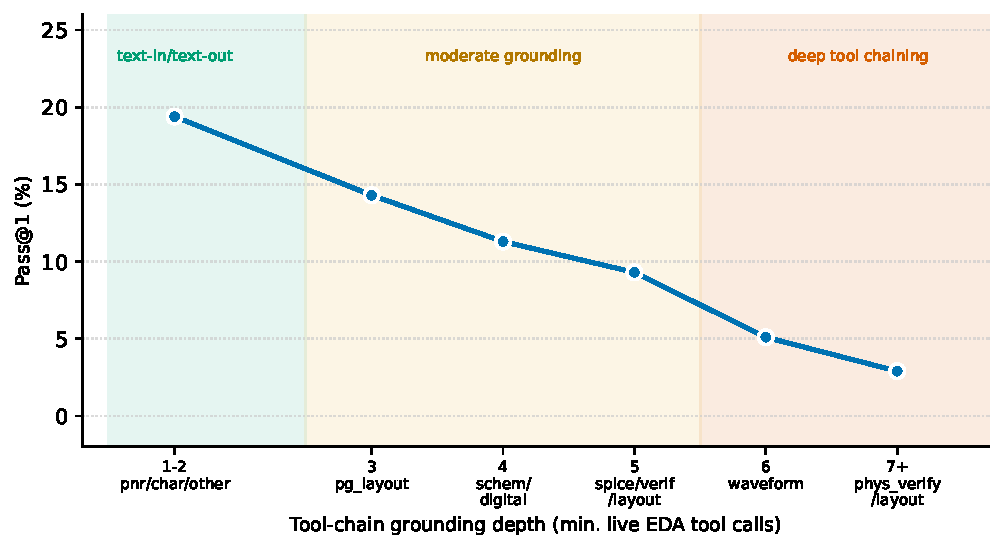
\includegraphics[width=\linewidth]{figures/grounding_depth.pdf}
\caption{Pass@1 by grounding-depth bin (domains grouped by our own annotation; the binning is a design choice, not a measured quantity). The ordering is descriptive: because depth is assigned by domain label, this figure does not by itself establish a causal or monotone relationship. Per-bin values are the means of the domains in Table~\ref{tab:main-results}.}
% \caption{按接地深度分箱的 Pass@1（分箱由我们手工标注，属设计选择而非测量量）。该排序是描述性的：
% 深度由领域标签指定，因此本图本身不能确立因果或严格单调关系。每箱取值见
% 表~\ref{tab:main-results} 中对应领域的均值。}
\label{fig:grounding-depth}
\end{figure}

\subsection{Trace Anatomy: A Pilot Study}
\label{sec:trace-anatomy}
% \subsection{轨迹解剖：试点研究}

To characterise \emph{how} runs behave rather than only whether they pass, we
instrumented 48 archived pilot runs (2026-11-03--11-06; 47 with a non-empty Cline
session log; 207\,MB, 1.21M events) and parsed every tool call, iteration and
termination record. This sample carries \emph{no judge verdict}---the pass/fail
labels live only in the batch runner---so the following are behavioural
statistics, not outcome attributions, and they are not extrapolated to the
\Neval{}-run evaluation.

\begin{itemize}
    \item \textbf{Effort.} The median run issues 26.5 tool calls (IQR 13.8--38.0,
    max 97) across 20.5 agent iterations (IQR 9.0--32.5), and runs for a median
    of 1{,}047\,s (IQR 552--1{,}495). Effort is therefore substantial but not
    unbounded: the deep-grounding tasks do not fail because the agent refuses to
    try.
    % \textbf{投入。} 中位 run 发出 26.5 次工具调用（IQR 13.8--38.0，最大 97），跨 20.5 轮
    % 迭代（IQR 9.0--32.5），中位耗时 1,047 秒（IQR 552--1,495）。投入可观但并非无界：
    % 深度接地任务失败并非因为智能体不肯尝试。
    \item \textbf{Tool mix.} Across 1{,}371 tool calls, 41.2\% go through the MCP
    bridge (\texttt{eda\_flow\_\_*}, \texttt{pyAether\_MCP\_server\_\_*}) and 58.8\%
    to built-in file/search/shell tools; \texttt{read\_files} alone is 28.8\% of
    all calls. The agent spends the plurality of its steps \emph{reading}, not
    driving EDA tools---consistent with an observation bottleneck rather than an
    action bottleneck.
    % \textbf{工具构成。} 1,371 次工具调用中 41.2\% 走 MCP 网桥，58.8\% 为内置文件/搜索/shell；
    % 单 read_files 占 28.8%。智能体的多数步骤用于\emph{读}而非驱动 EDA 工具——与"瓶颈在观测
    % 而非动作"一致。
    \item \textbf{Termination.} 27 runs end normally (\texttt{finishReason=completed}),
    6 terminate with an \texttt{error} event, 3 were aborted by a human, and 11
    archives are truncated mid-stream (5 of them cut at 1{,}794--1{,}799\,s, i.e.\
    within 6\,s of a 30-minute mark). Truncation inflates apparent "no-output"
    rates, which is why we report run-level status separately from trace-level
    termination.
    % \textbf{终止形态。} 27 个 run 正常结束，6 个以 error 事件终止，3 个被人为中止，
    % 11 份归档在流中被截断（其中 5 份截在 1,794--1,799 秒，距 30 分钟整点 <6 秒）。
    % 归档截断会抬高表面上的"无输出"比例——这也是我们把 run 级状态与轨迹级终止分开报告的原因。
    \item \textbf{Two harness artefacts.} One case shows the wrapper failing before
    the agent started (\texttt{o-approve: command not found}) while its
    \texttt{outputs/} directory still contained files, and one run logged 2{,}565\,s
    despite the nominal 2{,}400\,s timeout. Both are harness-side defects that the
    batch-level status alone would mis-attribute to the model; they motivate the
    per-run triage tool shipped with the benchmark.
    % \textbf{两个框架侧缺陷。} 一例显示 wrapper 在 agent 启动前就失败
    % （o-approve: command not found），但 outputs/ 里仍留有文件；另一例记录了 2,565 秒，
    % 超过名义上的 2,400 秒超时。二者都是框架侧缺陷——只看批次级状态会把它们错记为模型问题；
    % 这也是我们随基准发布逐 run 归因工具的原因。
\end{itemize}

\subsection{Distribution Analysis}
\label{sec:distribution}
% \subsection{分布分析}

\bench's domain distribution (Figure~\ref{fig:domain-distribution}) reflects real engineering practice, as discussed in Section~\ref{sec:domain-coverage}. This is a \emph{feature} of trace-based benchmark construction: the distribution reflects actual agent usage patterns, not synthetic task design.
% \bench{} 的领域分布（图~\ref{fig:domain-distribution}）反映了真实工程实践，如第~\ref{sec:domain-coverage}~节所述。这是基于轨迹构建基准的一个"特性"：分布反映真实的智能体使用模式，而非合成的任务设计。

\subsection{Threats to Validity}
\label{sec:threats}
% \subsection{有效性威胁}

\textbf{Domain imbalance.} Counting the \Neval{} evaluated runs, the top three domains hold 44.3\% and digital-front domains 12.8\%. This reflects real usage but may bias aggregate metrics toward analog-friendly capabilities.
% \textbf{领域失衡。} 按 \Neval{} 个已评测 run 计，前三个领域占 44.3\%，数字前端类领域占 12.8\%。这反映了真实使用情况，但可能使聚合指标偏向对模拟友好的能力。

\textbf{Single backbone.} All \Neval{} runs use one backbone (DeepSeek-V4-Pro). Claims about ``the best'' or about model scaling are therefore not supported by our own data; RQ3 is reported as an open question (Section~\ref{sec:model-scaling}).
% \textbf{单一骨干。} \Neval{} 个 run 全部使用同一骨干（DeepSeek-V4-Pro）。因此"最优模型"或"模型扩展"的论断不由我们自己的数据支撑；RQ3 作为开放问题报告。

\textbf{Frozen snapshot.} Results are tied to the 2026-11-09 snapshot of \Neval{} runs over the Full set, which has since grown to \Ntasks{} cases. Adding cases changes the domain mix and the achievable score; comparisons across snapshots are not valid unless the snapshot is pinned. The Lite set (\LiteSet{} tasks, Appendix) is fixed to support reproducible daily evaluation.
% \textbf{冻结快照。} 结果绑定在 2026-11-09 的 \Neval{}-run 快照上（基于 Full 集），而 Full 集已增长至 \Ntasks{} 个案例。
% 新增案例会改变领域构成与可达分数；除非固定快照，跨快照比较无效。Lite 集（\LiteSet{} 个任务，见附录）已固定，以支持可复现的日常评测。

\textbf{Trace sample bias.} The behavioural statistics in Section~\ref{sec:trace-anatomy} come from 47 archived pilot logs, not from the \Neval{}-run batch: archived traces are those that survived local retention, and 11 of them are truncated. They describe mechanics (effort, tool mix, termination), not pass rates.
% \textbf{轨迹样本偏差。} 第~\ref{sec:trace-anatomy}~节的行为学统计来自 47 份归档 pilot 日志，而非 \Neval{}-run 批次：
% 能归档的是本地留存下来的轨迹，且其中 11 份被截断。它们描述机制（投入、工具构成、终止形态），不描述通过率。

\textbf{Single tool ecosystem.} All tasks use commercial EDA tools (Empyrean Aether, Cadence, Synopsys) accessible via a single EDA server. Generalization to open-source EDA (Yosys, OpenROAD, Magic) is not evaluated.
% \textbf{单一工具生态。} 所有任务使用商业 EDA 工具（华大九天 Aether、Cadence、Synopsys），通过单一 EDA 服务器访问。对开源 EDA（Yosys、OpenROAD、Magic）的泛化能力未作评估。

\textbf{Single agent harness.} We evaluate only Cline; other agent frameworks (SWE-agent, OpenHands, AutoGPT) may perform differently. However, the anti-leakage protocol and MCP bridge are agent-agnostic.
% \textbf{单一智能体框架。} 我们只评测了 Cline；其他智能体框架（SWE-agent、OpenHands、AutoGPT）可能表现不同。但防泄题协议与 MCP 网桥是与具体智能体无关的。

\textbf{Trace provenance.} Tasks are derived from real user sessions, which may contain company-specific conventions, PDK-specific constraints, or tool-version-specific behaviors that limit generalizability.
% \textbf{轨迹来源。} 任务源于真实用户会话，可能包含公司专属约定、PDK 专属约束或工具版本专属行为，从而限制泛化性。
